\documentclass[xcolor=table, aspectratio=169, bigger]{beamer}

\usepackage{shyne}

% Theme settings
\setbeamertemplate{navigation symbols}{}

\usetheme{Madrid}
\usefonttheme{structurebold}
\usefonttheme[onlymath]{serif}

\AtBeginSection[]
{ 	\begin{frame}{}

	{
	\usebeamerfont{frametitle}
	\begin{beamercolorbox}
		[wd={\textwidth}, center, sep=.2in, rounded=true, shadow=true]
		{frametitle}
	Week \thesection\\  \secname 
	\end{beamercolorbox}
	}
	
	\end{frame} 
}

\AtBeginSubsection[]
{ 	\begin{frame}{}

	{
	\usebeamerfont{frametitle}
	\begin{beamercolorbox}
		[wd={\textwidth}, center, sep=.2in, rounded=true, shadow=true]
		{frametitle}
	Section \thesection .\thesubsection\\  \subsecname 
	\end{beamercolorbox}
	}
	
	\end{frame} 
}


\title[Week 1]{Stat 201: Statistics I\\ Week 1 }
\author[M. Shyne]{}
\institute[Metro State]{
\includegraphics[width=1.75in]{../images/metro_logo}}
\date[11/24/2018]{
\\ \bigskip \bigskip 
\includegraphics[width=.4in]{../images/cc_big}}


\begin{document}
 
\frame{\titlepage}

%
% Week 1
%
\section{Introduction to Statistics and Data}

%
% Section 1.1
%
\subsection{Statistical and Critical Thinking}

%%%%%%%%%%
\begin{frame}{Why study statistics?}
\begin{block}{}
``Statistics is the language of science."
\end{block}

\pause
\begin{block}{}
Statistics is also the language of...
\begin{itemize}
\item Politics (both campaigns and public policy)
\item Economics
\item Business
\item Psychology and social sciences
\item \ldots
\end{itemize}

\end{block}
\end{frame}

%%%%%%%%%%
\begin{frame}{Why study statistics? (cont)}
\begin{block}{}
Some of us will \bt{do} statistics. \\
\medskip\pause
Statistics are an important component of many of the fastest growing careers. As of November 2018,
\begin{itemize}
\item Statistician is the second fastest growing career in Minnesota.
\pause\item Computer and information research scientist, operations research analyst, actuary and market research analyst are all in the top 20.
\end{itemize}
\end{block}

\pause

\begin{block}{}
All of us are \bt{consumers} of statistics.\\
\pause
\begin{itemize}
\item Many fields make extensive use of statistics and research to make decisions.
\pause\item Much of the news and information we encounter on a daily basis involves statistics.
\end{itemize}
\end{block}

\end{frame}


%%%%%%%%%%
\begin{frame}{What is statistics?}

\begin{block}{}
\bt{Statistics} is the science of using data from samples to learn about populations.
\end{block}

\pause
\begin{block}{}
\bt{Data} are collections of observations, such as measurements, biographical information or survey responses.
\end{block}

\pause
\begin{block}{}
A \bt{population} is any group that we are interested in knowing something about.
\end{block}

\pause
\begin{block}{}
A \bt{sample} is a subset of a population used to represent the whole population.
\end{block}

\pause
\begin{block}{}
A \bt{census} is when data is collected from \emph{every} member of a population.
\end{block}


\end{frame}


%%%%%%%%%%
\begin{frame}{Population and sample examples}

\begin{exampleblock}{Example}
\begin{center}
\tabspacemed
\begin{tabular}{p{2.5in} | p{2.5in} }
Population & Sample\\
\hline
The entire population of the United States & Respondents to an internet survey\pause\\
Males over 40 who have high blood pressure & High blood pressure patients in a clinical trial\pause\\

Students enrolled at Metro State in 2017 & You (the students in this class)\pause\\
Statistics classes in Minnesota & The summer semester statistics classes at Metro State\\
\end{tabular}
\end{center}
\end{exampleblock}

\end{frame}


%%%%%%%%%%
\begin{frame}{Statistical process}
\begin{block}{}
\begin{itemize}
\item<1-> \bt{Prepare}
\begin{itemize}
\item<2-> Identify research question
\item<2-> Design the study
\item<2-> Collect data
\end{itemize}
\item<1-> \bt{Analyze}
\begin{itemize}
\item<3-> Graph and explore the data
\item<3-> Produce informative summaries of data
\item<3-> Conduct statistical tests or other analyses
\end{itemize}
\item<1-> \bt{Conclude}
\begin{itemize}
\item<4-> Report results in the context of the research question
\end{itemize}
\end{itemize}
\end{block}

\end{frame}


%%%%%%%%%%
\begin{frame}{Possible pitfalls: Prepare}
\begin{block}{}
\begin{itemize}
\item What is the goal of the study? Is the research question clear?
\item What do the data mean? Can the data answer the research question?
\item Are the data or is the study from a source with a special interest so that there is pressure to obtain results that are favorable to the source?
\item What sampling method was used? Were the data collected in a way that is biased?
\item Are the data self-reported?
\item Is the sample size adequate?
\item What questions were used to elicit responses?
\end{itemize}
\end{block}
\end{frame}

%%%%%%%%%%
\begin{frame}{Can the data answer the research question?}

\begin{exampleblock}{Example}
Suppose a group of researchers wants to study the association between intelligence and grades. So, they collect the GPAs of a random sample of students and measure their skull circumference\ldots\\
\end{exampleblock}
\pause
\begin{alertblock}{Note}
This is not a completely made up example. Phrenology was the study of skull sizes and shapes, and was used as recently as the early 20th century to ``prove" that non-white races were inferior and to diagnose mental illness.
\end{alertblock}
\end{frame}

%%%%%%%%%%
\begin{frame}
\frametitle{Are the data from a source with a special interest?}
\begin{exampleblock}{Example}
According to an article in the NY Daily News from June, 2014, titled, ``Strip down: Sleeping naked is good for your relationship, survey says" (\href{http://www.nydailynews.com/life-style/health/survey-sleeping-naked-good-relationships-article-1.1849491}{link)}\ldots\\
\medskip
From a survey of 1000 British couples, ``57\% of those who reported sleeping in the buff said they felt happy, compared with 48\% of pajama wearers and 43\% of nightie wearers."\\

\begin{itemize}
\pause\item The survey was conducted by Cotton USA.
\end{itemize}
\end{exampleblock}

\end{frame}

%%%%%%%%%%
\begin{frame}{Were the data collected in a way that is biased?}

\begin{block}{}
A \bt{voluntary response sample} (or \bt{self-selected sample}) is one in which the respondents themselves decide whether to be included. 
\end{block}

\pause
\begin{exampleblock}{Example}
\begin{itemize}
\item Call-in polls to radio or tv stations
\item Online surveys
\item Internet comment or review sections
\item Trending on twitter
\end{itemize}
\end{exampleblock}
\end{frame}

%%%%%%%%%%
\begin{frame}{Other issues with prepare step}
\begin{block}{}
\begin{itemize}
\item \bt{Self-reported results} are data provided by the subjects of a study, rather than measured directly. Self-reported data can be inaccurate and/or imprecise.
\pause\item \bt{Sample size} is important. Be wary of results drawn from very small samples.
\pause\item \bt{Loaded questions} are those designed to elicit a particular response or to influence the subject.
\begin{itemize}
\item Also known as: push polls
\end{itemize}
\pause\item The \bt{order of questions} can influence responses.
\end{itemize}
\end{block}

\end{frame}

%%%%%%%%%%
\begin{frame}{Possible pitfalls: Analyze}
 
\begin{block}{}
\begin{itemize}
\item Are there any outliers?
\item Are there missing data?
\item How are the data distributed?
\item Was an appropriate test used?
\end{itemize}
\end{block}

\begin{block}{}
The rest of the course is primarily focused in the analyze step. We will discuss most of these issues as we go.
\end{block}
\end{frame}

%%%%%%%%%%
\begin{frame}{Are there missing data?}

\begin{block}{}
Missing data can result from subjects dropping out of the study or skipping scheduled data collection appointments. Almost every study has to deal with missing data. The existence of missing data is not necessarily concerning unless,
\begin{itemize}
\item A large proportion of the the original sample is missing or has missing data
\item The pattern of missing data is biased (known as \bt{informative missingness})
\end{itemize}
\end{block}

\pause
\begin{exampleblock}{Example}
An experimental drug trial with a large proportion of drop-outs from group taking the new drug would be cause for concern. It could be caused by subjects who are experiencing severe side effects and/or ineffective treatment leaving the study. Any conclusions drawn only from the remaining subjects would then be misleading.
\end{exampleblock}
\end{frame}


%%%%%%%%%%
\begin{frame}
\frametitle{Possible pitfalls: Conclude}

\begin{block}{}
\begin{itemize}
\item Do the results have statistical significance? Do the results have practical significance?
\item Are the conclusions justified by the data?
\item Is there a confusion of precision for accuracy?
\item Are percentages used clearly?
\end{itemize}
\end{block}

\end{frame}

%%%%%%%%%%
\begin{frame}{Are the results significant?}
\begin{block}{}
\begin{itemize}
\item Do the results have statistical significance?
\begin{itemize}
\item Statistical significance is a measure of how unlikely observed results are given certain assumptions.
\item Statistical significance is determined by many factors, including study design.
\end{itemize}
\pause\item Do the results have practical significance?
\begin{itemize}
\item Do the results matter?
\end{itemize}
\end{itemize}
\end{block}

\pause
\begin{exampleblock}{Example}
A clinical trial shows a new drug lowers systolic blood pressure by an average of 3 mmHg. Results might be statistically significant, but are probably not practically significant.
\end{exampleblock}
\end{frame}

%%%%%%%%%%
\begin{frame}{Are the conclusions justified by the data?}

\begin{block}{}
It is common to mistake an association or relationship between two factors for one factor causing the other.
\end{block}

\pause

\begin{alertblock}{!!!}
\Large Correlation does not imply causation.
\end{alertblock}

\pause
\begin{exampleblock}{Example}
Recall the sleeping naked study.\\
\medskip
Though the article made the claim that sleeping naked \bt{caused} happier relationships, the study merely pointed to an association.\\
\medskip
There are many other possible explanations for that association. This study alone does not provide evidence for which explanation is ``true".

\end{exampleblock}

\end{frame}


%%%%%%%%%%
\begin{frame}{Is there a confusion of precision for accuracy?}

\begin{block}{}
Precision is not the same thing as accuracy.
\end{block}

\begin{center}
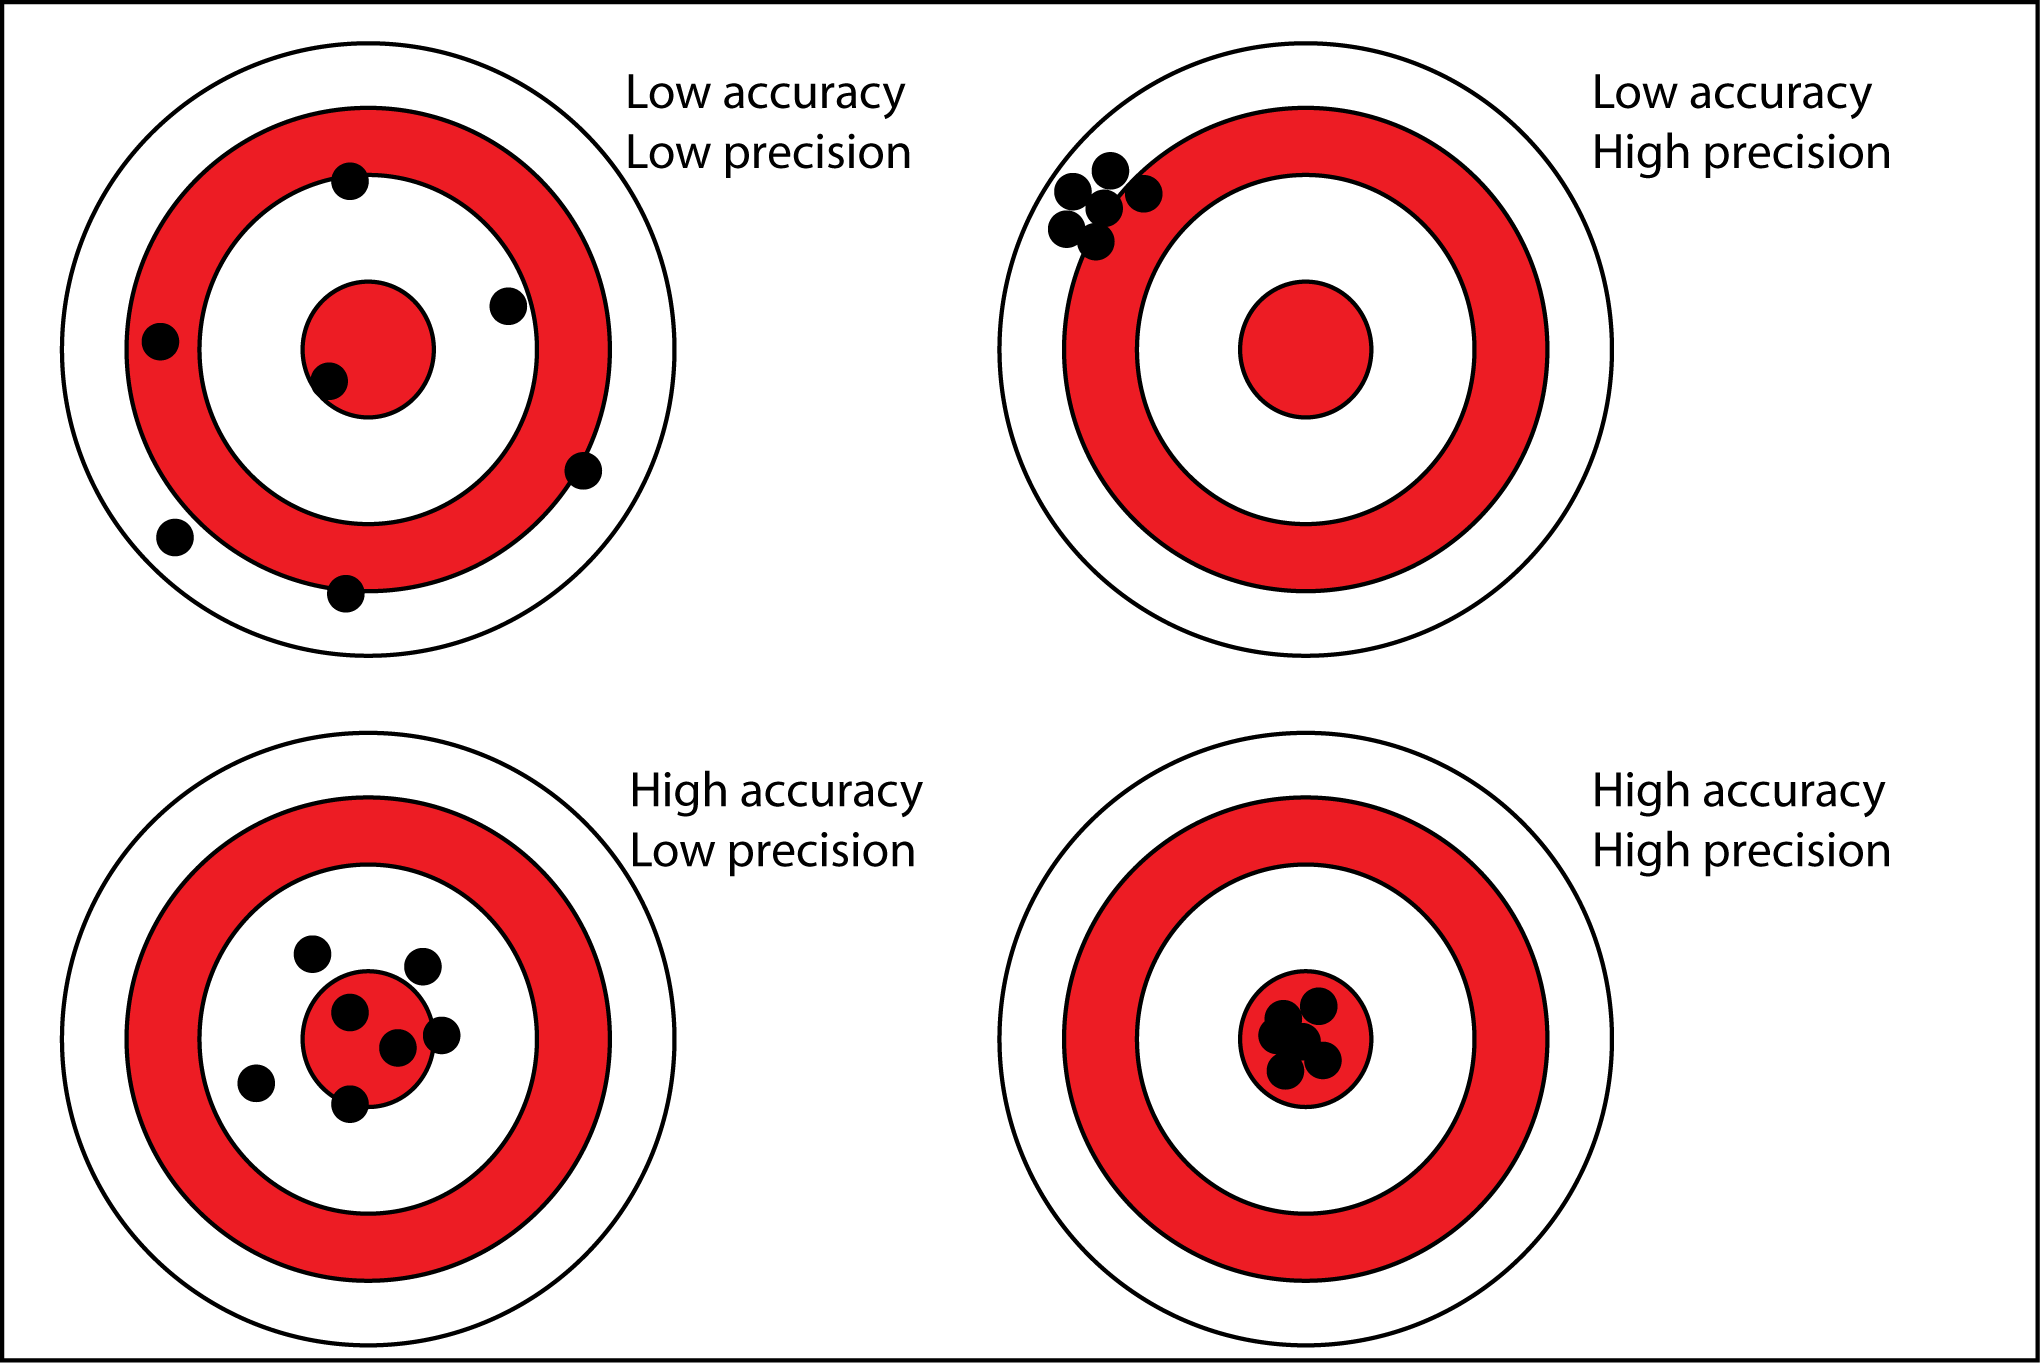
\includegraphics[width=3.5in]{../images/precision_accuracy}
\end{center}
\end{frame}

%%%%%%%%%%
\begin{frame}{Are percentages used clearly?}

\begin{block}{}
Sometimes percentages are used in confusing ways. Remember, 100\% of a thing is all of it. Percentages above 100, or phrases like ``a reduction of 100\%", do not always have clear meanings. 
\end{block}

\begin{exampleblock}{Example}
Suppose a company sold 10 widgets last year. This year they report an increase in widget sales of 150\%. How many widgets did they sell this year?
\begin{itemize}
\item Answers of 15 or 25 widgets could both be reasonably justified. 
\end{itemize}
\end{exampleblock}

\end{frame}

%%%%%%%%%%
\begin{frame}
\frametitle{Percentages: Review}

\begin{block}{}
\begin{itemize}
\item A \bt{percentage} is number describing a proportion as an amount out of 100 (per cent).
\pause
\item We can also describe a \bt{proportion} as a fraction of 1.
\[\ds \frac {50}{100} = \frac 1 2 \quad \implies \quad 50\% = .50\]
\pause
\item 100\% represents a whole, just as for proportions 1 represents a whole.
\pause
\item It often doesn't make sense to talk about percentages greater than 100\%.
\end{itemize}
\end{block}
\end{frame}

%%%%%%%%%%
\begin{frame}
\frametitle{Percentages: Calculations}
\begin{exampleblock}{}
To convert from percentage to proportion, divide by 100:
\[56\% \quad \implies \quad \frac {56}{100} = 0.56\]

To convert from proportion to percentage, multiply by 100:
\[\frac 5 8 = 0.625 \quad \implies \quad 0.625 \times 100 = 62.5\%\]

To find the quantity a percentage represents:
\[\text{13\% of 264}\quad \implies \quad \frac {13}{100} \times 264 = 34.32\]

To find the percentage a quantity represents:
\[\text{135 out of 475} \quad \implies \quad \frac {135}{475} \times 100 = 28.42\ldots \%\]
\end{exampleblock}
\end{frame}

%%%%%%%%%%
\begin{frame}<handout:0>{Group work}
\begin{block}{}

\begin{itemize}
\item Get into groups of 2 - 4
\item For each question, read the scenario. Discuss and note some answers to part (a).
\item Don't worry about getting exactly the right answers. Thinking about and discussing the question is more important.
\end{itemize}
\end{block}
\end{frame}


%
% Section 1.2
%
\subsection{Introduction to Data}

%%%%%%%%%%
\begin{frame}
\frametitle{Parameters and statistics}

\begin{block}{}
A \bt{parameter} is a value describing an aspect of a population.
\end{block}
\pause
\begin{block}{}
A \bt{statistic} is a value describing an aspect of a sample.
\end{block}
\pause
\begin{exampleblock}{Example}
\begin{itemize}
\item The average height of adult men in the U.S. is 72 inches: \bt{Parameter}

\item The average height of 30 randomly selected male Metro State students is 68.5 inches: \bt{Statistic}
\end{itemize}
\end{exampleblock}

\end{frame}

%%%%%%%%%%
\begin{frame}{Organization of data}

\begin{table}[ht]
\centering
\begin{tabular}{rrlrrr}
  \hline
ID & AGE & SEX & LENGTH & WEIGHT & CHEST \\ 
  \hline
1030 & 21 & Male & 61.0 & 150 & 34.0 \\ 
  1004 & 115 & Male & 72.0 & 348 & 49.0 \\ 
  1050 & 17 & Female & 52.5 & 76 & 28.0 \\ 
  1040 & 58 & Male & 70.5 & 365 & 50.0 \\ 
  1020 & 177 & Male & 72.0 & 436 & 48.0 \\ 
  1010 & 53 & Female & 58.0 & 144 & 31.0 \\ 
   \hline
\end{tabular}
\end{table}

\begin{block}{}
Data is often presented as a table or \bt{data matrix}.
\begin{itemize}
\pause\item Each row represents one \bt{case} or \bt{subject}. Also known as a \bt{unit of observation}.
\pause\item Each column represents one characteristic or \bt{variable}. Also known as a \bt{factor}.
\pause\item Ideally, a data matrix will be accompanied by a codebook, a document that explains each variable.
\end{itemize}
\end{block}

\end{frame}


%%%%%%%%%%
\begin{frame}
\frametitle{Types of data}

\begin{block}{}
\bt{Quantitative} data are numbers representing amounts, sizes, time or other measurements.\\
Also known as: Numeric
\end{block}

\begin{exampleblock}{Example}
Class size, height, age, systolic blood pressure, temperature
\end{exampleblock}

\pause

\begin{block}{}
\bt{Categorical} data are values representing groups or categories.
\begin{itemize}
\item Also known as: qualitative, attribute
\end{itemize}
\end{block}

\begin{exampleblock}{Example}
Gender, state of residence, football player's numbers, pain scale
\end{exampleblock}

\end{frame}

%%%%%%%%%%
\begin{frame}{Types of data: Quantitative}
\begin{block}{}
\bt{Discrete} data have a finite, or countably infinite, number of possible values. There are gaps in the possible values.
\end{block}

\begin{exampleblock}{Example}
Class size: can't have a class size of 22.5
\end{exampleblock}
\pause
\begin{block}{}
\bt{Continuous} data have an infinite number of possible values. There are no gaps in possible values.
\end{block}

\begin{exampleblock}{Example}
Height: a height of 70.2641... inches is possible (not necessarily useful, but possible)
\end{exampleblock}

\end{frame}

%%%%%%%%%%
\begin{frame}{Levels of measurement}
\begin{block}{}
\begin{itemize}
\item Nominal
\item Ordinal
\item Interval
\item Ratio
\end{itemize}
\end{block}
\end{frame}


%%%%%%%%%%
\begin{frame}{Levels of measurement: Nominal}
\begin{block}{}
The \bt{nominal} level of measurement is categorical data that are names or labels for groups or categories. There is no reasonable order or ranking to the categories.
\end{block}
\pause
\begin{exampleblock}{Example}
\begin{itemize}
\item Gender: \emph{male} or \emph{female}
\item State of residence: \emph{Minnesota}, \emph{Wisconsin}, etc.
\end{itemize}
\end{exampleblock}
\pause
\begin{alertblock}{Hint}
The root word \emph{nom} means ``name''.
\end{alertblock}
\end{frame}

%%%%%%%%%%
\begin{frame}
\frametitle{Levels of measurement: Ordinal}
\begin{block}{}
The \bt{ordinal} level of measure is categorical data that are naturally ordered or ranked.
\end{block}
\pause
\begin{exampleblock}{Example}
\begin{itemize}
\item Pain scale: \emph{No pain} $<$ \emph{Moderate pain} $<$ \emph{Heavy pain}
\item Grades: \emph A $>$ \emph B $>$ \emph C $>$ \emph D $>$ \emph F
\end{itemize}
\end{exampleblock}
\end{frame}

%%%%%%%%%%
\begin{frame}
\frametitle{Levels of measurement: Interval}
\begin{block}{}
The \bt{interval} level of measurement is quantitative data where\\ the difference between values has meaning but where there is no natural ``zero''.
\end{block}
\pause
\begin{exampleblock}{Example}
\begin{itemize}
\item Temperature: The difference between 101\textdegree F and 98.6\textdegree F is meaningful, but 0\textdegree F does not mean no temperature.
\item Year: 2017 is four years after 2013, but year 0 does not mean no years.
\end{itemize}
\end{exampleblock}
\end{frame}

%%%%%%%%%%
\begin{frame}
\frametitle{Levels of measurement: Ratio}
\begin{block}{}
The \bt{ratio} level of measurement is quantitative data where the difference between values and relative sizes of values have meaning. There is a natural ``zero''.
\end{block}
\pause
\begin{exampleblock}{Example}
\begin{itemize}
\item Age: Someone who is 40 years old is \emph{twice} as old as someone who is 20 years old. Zero does mean no age.

\item Height: A tree that is 10 feet tall is \emph{one third} as tall as a tree that is 30 feet tall. Zero does mean no height.
\end{itemize}

\end{exampleblock}
\end{frame}

%%%%%%%%%%
\begin{frame}<handout:0>{Group work}
\begin{block}{}
\begin{itemize}
\item Get back into your groups.
\item Discuss and note some answers to part (b) for each question.
\item Remember, getting exactly the right answer is less important than the discussion.
\end{itemize}
\end{block}
\end{frame}

\end{document}